% Editable AST for Example 1.
% Compile with: pdflatex -output-directory=build ast_example1_editable.tex
\documentclass[tikz,border=4pt]{standalone}
\usepackage{amsmath,amssymb}
\usepackage{tikz}

\begin{document}
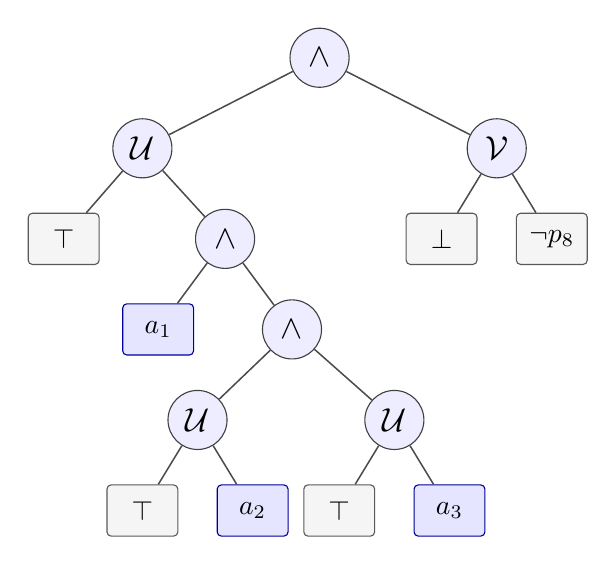
\begin{tikzpicture}[
  x=1cm,
  y=1cm,
  edge/.style={draw=black!70, line width=0.55pt},
  operator/.style={
    circle,
    draw=black!75,
    fill=blue!7,
    minimum size=7.5mm,
    inner sep=0pt,
    font=\large
  },
  action/.style={
    rounded corners=1.5pt,
    draw=blue!60!black,
    fill=blue!10,
    minimum width=9mm,
    minimum height=6.5mm,
    inner sep=1pt,
    font=\normalsize
  },
  literal/.style={
    rounded corners=1.5pt,
    draw=black!65,
    fill=black!4,
    minimum width=9mm,
    minimum height=6.5mm,
    inner sep=1pt,
    font=\normalsize
  }
]

% Node coordinates are deliberately explicit so that the layout is easy to edit.
% Formula after rewriting:
% [top U (a1 AND ((top U a2) AND (top U a3)))]
% AND [bottom V (not p8)].

\node[operator] (root) at (0,0) {$\wedge$};

\node[operator] (u0) at (-2.25,-1.15) {$\mathcal U$};
\node[operator] (v0) at ( 2.25,-1.15) {$\mathcal V$};

\node[literal]  (top0) at (-3.25,-2.30) {$\top$};
\node[operator] (and0) at (-1.20,-2.30) {$\wedge$};
\node[literal]  (bot0) at ( 1.55,-2.30) {$\bot$};
\node[literal]  (notp8) at ( 2.95,-2.30) {$\neg p_8$};

\node[action]   (a1) at (-2.05,-3.45) {$a_1$};
\node[operator] (and1) at (-0.35,-3.45) {$\wedge$};

\node[operator] (u2) at (-1.55,-4.60) {$\mathcal U$};
\node[operator] (u3) at ( 0.95,-4.60) {$\mathcal U$};

\node[literal] (top2) at (-2.25,-5.75) {$\top$};
\node[action]  (a2)   at (-0.85,-5.75) {$a_2$};
\node[literal] (top3) at ( 0.25,-5.75) {$\top$};
\node[action]  (a3)   at ( 1.65,-5.75) {$a_3$};

\draw[edge] (root) -- (u0);
\draw[edge] (root) -- (v0);
\draw[edge] (u0) -- (top0);
\draw[edge] (u0) -- (and0);
\draw[edge] (v0) -- (bot0);
\draw[edge] (v0) -- (notp8);
\draw[edge] (and0) -- (a1);
\draw[edge] (and0) -- (and1);
\draw[edge] (and1) -- (u2);
\draw[edge] (and1) -- (u3);
\draw[edge] (u2) -- (top2);
\draw[edge] (u2) -- (a2);
\draw[edge] (u3) -- (top3);
\draw[edge] (u3) -- (a3);

\end{tikzpicture}
\end{document}
